% Options for packages loaded elsewhere
\PassOptionsToPackage{unicode}{hyperref}
\PassOptionsToPackage{hyphens}{url}
%
\documentclass[
]{article}
\usepackage{amsmath,amssymb}
\usepackage{iftex}
\ifPDFTeX
  \usepackage[T1]{fontenc}
  \usepackage[utf8]{inputenc}
  \usepackage{textcomp} % provide euro and other symbols
\else % if luatex or xetex
  \usepackage{unicode-math} % this also loads fontspec
  \defaultfontfeatures{Scale=MatchLowercase}
  \defaultfontfeatures[\rmfamily]{Ligatures=TeX,Scale=1}
\fi
\usepackage{lmodern}
\ifPDFTeX\else
  % xetex/luatex font selection
\fi
% Use upquote if available, for straight quotes in verbatim environments
\IfFileExists{upquote.sty}{\usepackage{upquote}}{}
\IfFileExists{microtype.sty}{% use microtype if available
  \usepackage[]{microtype}
  \UseMicrotypeSet[protrusion]{basicmath} % disable protrusion for tt fonts
}{}
\makeatletter
\@ifundefined{KOMAClassName}{% if non-KOMA class
  \IfFileExists{parskip.sty}{%
    \usepackage{parskip}
  }{% else
    \setlength{\parindent}{0pt}
    \setlength{\parskip}{6pt plus 2pt minus 1pt}}
}{% if KOMA class
  \KOMAoptions{parskip=half}}
\makeatother
\usepackage{xcolor}
\usepackage[margin=1in]{geometry}
\usepackage{longtable,booktabs,array}
\usepackage{calc} % for calculating minipage widths
% Correct order of tables after \paragraph or \subparagraph
\usepackage{etoolbox}
\makeatletter
\patchcmd\longtable{\par}{\if@noskipsec\mbox{}\fi\par}{}{}
\makeatother
% Allow footnotes in longtable head/foot
\IfFileExists{footnotehyper.sty}{\usepackage{footnotehyper}}{\usepackage{footnote}}
\makesavenoteenv{longtable}
\usepackage{graphicx}
\makeatletter
\def\maxwidth{\ifdim\Gin@nat@width>\linewidth\linewidth\else\Gin@nat@width\fi}
\def\maxheight{\ifdim\Gin@nat@height>\textheight\textheight\else\Gin@nat@height\fi}
\makeatother
% Scale images if necessary, so that they will not overflow the page
% margins by default, and it is still possible to overwrite the defaults
% using explicit options in \includegraphics[width, height, ...]{}
\setkeys{Gin}{width=\maxwidth,height=\maxheight,keepaspectratio}
% Set default figure placement to htbp
\makeatletter
\def\fps@figure{htbp}
\makeatother
\setlength{\emergencystretch}{3em} % prevent overfull lines
\providecommand{\tightlist}{%
  \setlength{\itemsep}{0pt}\setlength{\parskip}{0pt}}
\setcounter{secnumdepth}{-\maxdimen} % remove section numbering
\usepackage{booktabs}
\usepackage{longtable}
\usepackage{array}
\usepackage{multirow}
\usepackage{wrapfig}
\usepackage{float}
\usepackage{colortbl}
\usepackage{pdflscape}
\usepackage{tabu}
\usepackage{threeparttable}
\usepackage{threeparttablex}
\usepackage[normalem]{ulem}
\usepackage{makecell}
\usepackage{xcolor}
\ifLuaTeX
  \usepackage{selnolig}  % disable illegal ligatures
\fi
\usepackage{bookmark}
\IfFileExists{xurl.sty}{\usepackage{xurl}}{} % add URL line breaks if available
\urlstyle{same}
\hypersetup{
  pdftitle={Final\_Project Report},
  pdfauthor={Ananya, Rosie, Sameer},
  hidelinks,
  pdfcreator={LaTeX via pandoc}}

\title{Final\_Project Report}
\author{Ananya, Rosie, Sameer}
\date{2025-04-04}

\begin{document}
\maketitle

\section{Introduction}\label{introduction}

\subsection{Why are we interested in Tidal
Power?}\label{why-are-we-interested-in-tidal-power}

\subsubsection{Relevance to our fields of studies and
interests:}\label{relevance-to-our-fields-of-studies-and-interests}

Our group is made up with students from Coastal Marine Systems and
Energy concentrations under the MEM program, and we decided that this
topic covered the fields of interests for all of our group members.

\subsubsection{Great Potential of Tidal
Energy:}\label{great-potential-of-tidal-energy}

Clean \& Sustainable Energy Source:\\
- Tidal power is a renewable energy that produces zero greenhouse gas
emissions. - Unlike traditional hydro power, tidal energy does not
require dams or large reservoirs, making it more environmentally
friendly.

High Energy Density \& Efficiency:\\
- Wind speeds shift, and sunlight fades, so such systems require storage
to sustain their service areas' electrical demand.\\
- By contrast, ocean currents are relatively constant, and some amount
of motion still occurs at all times.\\
- So, a tidal energy farm can provide continuous power without the need
for expensive battery or fuel cell storage.\\
- Tidal energy has a higher power capacity than many other renewable,
helping bridge the gap in clean energy demand.

Reliable \& Predictable:\\
- Unlike intermittent sources like wind and solar, tidal currents are
consistent and predictable, providing continuous power without heavy
reliance on storage.\\
- This reliability helps balance energy grids, complementing other
renewables during low-generation periods.

Growing U.S. Interest \& Investment:\\
- No commercially available sites right now in the US.\\
- There are Early projects in Maine and New York have successfully
tested tidal turbines.

\section{Project Overview:}\label{project-overview}

In this project, we are aiming to compare the Tidal Power Potential
across three sites in different latitudes and coastal areas with
different geographic and climatic conditions in the US. The tidal power
potential is assessed by:\\
- The Wave Energy Flux (Watts per square meter) = Wave Power Density
(Joules per cubic meter) * Wave Energy Period (seconds).\\
- Then in the Analysis below, we are going to compare the seasonal and
long term trends of the time series of the Wave Energy Flux that we
calculated.\\
- Then we will run models of prediction based on training and testing
datasets that we extracted in the original time series data.\\
- Then we compare the model forecasting results to see which site has
better model prediction results and higher/ more stable values (Wave
Energy Flux).

\section{Data selection}\label{data-selection}

We first picked 3 sites/ locations/ areas tend to be some of the
locations referred to for its tidal power potential in the general
Internet searches. These three sites are:\\
- Gulf of Maine (43.68° N, 69.77 ° W)\\
- \textasciitilde{} 3 km distance into ocean near Miami, Florida (25.74
° N, 80.11 ° W)\\
- Cook Inlet, Alaska (59.37° N, 152.64° W)

With the lat-long of these sites, we extracted raw data of 1979-2010
Wave Energy Density and Energy period data in NREL marine energy atlas:
\url{http://nrel.gov/marine-energy-atlas/data-viewer}

These areas are distinct by latitudes and longitudes, as well as
different coasts and climatic environments.

\section{Data Wrangling \& Initial
Analysis}\label{data-wrangling-initial-analysis}

\begin{itemize}
\tightlist
\item
  In general, we first calculated the Wave Energy Flux data based on the
  raw data we extracted.\\
\item
  Then the Wave Energy Flux datasets for all 3 sites' were aggregated to
  daily and monthly view (original series).\\
\item
  Then we split the current full dataset using 80/20 rule into training
  and testing datasets.\\
\item
  Then, we conducted the original time series analysis.\\
\item
  Then we ran various models to compare predicting/ forecasting
  performance on the Maine dataset.\\
\item
  Then we used the top 3 performance models (Arima + Fourier k-4, TBATs.
  and STL+ETS) for the other 2 sites Wave Energy Flux.
\item
  Compare Wave Energy Flux Results of the 3 sites and determine which
  site has more potential.
\end{itemize}

\begin{verbatim}
## [1] "/Users/sameerswarup/Documents/Duke MEM Classes/Spring 2025/Time Series Analysis for Energy/RStudio Outputs/Final_Project"
\end{verbatim}

\begin{verbatim}
## [1] "/Users/sameerswarup/Documents/Duke MEM Classes/Spring 2025/Time Series Analysis for Energy/RStudio Outputs/Final_Project/Code"
\end{verbatim}

\begin{verbatim}
## `summarise()` has grouped output by 'Year', 'Month'. You can override using the
## `.groups` argument.
## `summarise()` has grouped output by 'Year', 'Month'. You can override using the
## `.groups` argument.
## `summarise()` has grouped output by 'Year', 'Month'. You can override using the
## `.groups` argument.
\end{verbatim}

\begin{verbatim}
## `summarise()` has grouped output by 'Year'. You can override using the
## `.groups` argument.
## `summarise()` has grouped output by 'Year'. You can override using the
## `.groups` argument.
## `summarise()` has grouped output by 'Year'. You can override using the
## `.groups` argument.
\end{verbatim}

As a starter for looking at wave energy potential across the three
sites, we generated 3 summary statistics tables below for the monthly
mean wave power across each site (from January 1979 to December 2010).

\begin{longtable}[]{@{}ll@{}}
\caption{Data summary}\tabularnewline
\toprule\noalign{}
\endfirsthead
\endhead
\bottomrule\noalign{}
\endlastfoot
Name & maine\_monthly\_df\$monthly\_\ldots{} \\
Number of rows & 384 \\
Number of columns & 1 \\
\_\_\_\_\_\_\_\_\_\_\_\_\_\_\_\_\_\_\_\_\_\_\_ & \\
Column type frequency: & \\
numeric & 1 \\
\_\_\_\_\_\_\_\_\_\_\_\_\_\_\_\_\_\_\_\_\_\_\_\_ & \\
Group variables & None \\
\end{longtable}

\textbf{Variable type: numeric}

\begin{longtable}[]{@{}
  >{\raggedright\arraybackslash}p{(\columnwidth - 20\tabcolsep) * \real{0.1373}}
  >{\raggedleft\arraybackslash}p{(\columnwidth - 20\tabcolsep) * \real{0.0980}}
  >{\raggedleft\arraybackslash}p{(\columnwidth - 20\tabcolsep) * \real{0.1373}}
  >{\raggedleft\arraybackslash}p{(\columnwidth - 20\tabcolsep) * \real{0.0784}}
  >{\raggedleft\arraybackslash}p{(\columnwidth - 20\tabcolsep) * \real{0.0784}}
  >{\raggedleft\arraybackslash}p{(\columnwidth - 20\tabcolsep) * \real{0.0784}}
  >{\raggedleft\arraybackslash}p{(\columnwidth - 20\tabcolsep) * \real{0.0784}}
  >{\raggedleft\arraybackslash}p{(\columnwidth - 20\tabcolsep) * \real{0.0784}}
  >{\raggedleft\arraybackslash}p{(\columnwidth - 20\tabcolsep) * \real{0.0882}}
  >{\raggedleft\arraybackslash}p{(\columnwidth - 20\tabcolsep) * \real{0.0882}}
  >{\raggedright\arraybackslash}p{(\columnwidth - 20\tabcolsep) * \real{0.0588}}@{}}
\toprule\noalign{}
\begin{minipage}[b]{\linewidth}\raggedright
skim\_variable
\end{minipage} & \begin{minipage}[b]{\linewidth}\raggedleft
n\_missing
\end{minipage} & \begin{minipage}[b]{\linewidth}\raggedleft
complete\_rate
\end{minipage} & \begin{minipage}[b]{\linewidth}\raggedleft
mean
\end{minipage} & \begin{minipage}[b]{\linewidth}\raggedleft
sd
\end{minipage} & \begin{minipage}[b]{\linewidth}\raggedleft
p0
\end{minipage} & \begin{minipage}[b]{\linewidth}\raggedleft
p25
\end{minipage} & \begin{minipage}[b]{\linewidth}\raggedleft
p50
\end{minipage} & \begin{minipage}[b]{\linewidth}\raggedleft
p75
\end{minipage} & \begin{minipage}[b]{\linewidth}\raggedleft
p100
\end{minipage} & \begin{minipage}[b]{\linewidth}\raggedright
hist
\end{minipage} \\
\midrule\noalign{}
\endhead
\bottomrule\noalign{}
\endlastfoot
data & 0 & 1 & 8443.42 & 4897.73 & 1528.53 & 4458.87 & 7346.83 &
11155.54 & 28885.92 & ▇▆▂▁▁ \\
\end{longtable}

\section{Maine}\label{maine}

\#\#\#We will use Maine to test our various time series models. Using
accuracy metrics and plots we will choose the 3 best models and forecast
mean monthly wave power for Alaska and Florida.

\includegraphics{Data_Cleaning_files/figure-latex/unnamed-chunk-6-1.pdf}
\includegraphics{Data_Cleaning_files/figure-latex/unnamed-chunk-6-2.pdf}

\begin{quote}
Observations: Daily mean wave power appears to be highly volatile and
masked by noise, which might make it harder to model directly. On the
other hand, monthly mean wave power shows a clear seasonal structure
with regular peaks and dips, and consistent annual cycles across
decades. Moreover, the ACF plot for the daily wave power drops sharply
after lag 1, suggesting that past daily values don't carry much signal
for future values. For the monthly wave power, the ACF plot shows strong
seasonality with the wave pattern. The autocorrelation persists over
time, which will be ideal for ARIMA/SARIMA and other seasonal models.
\end{quote}

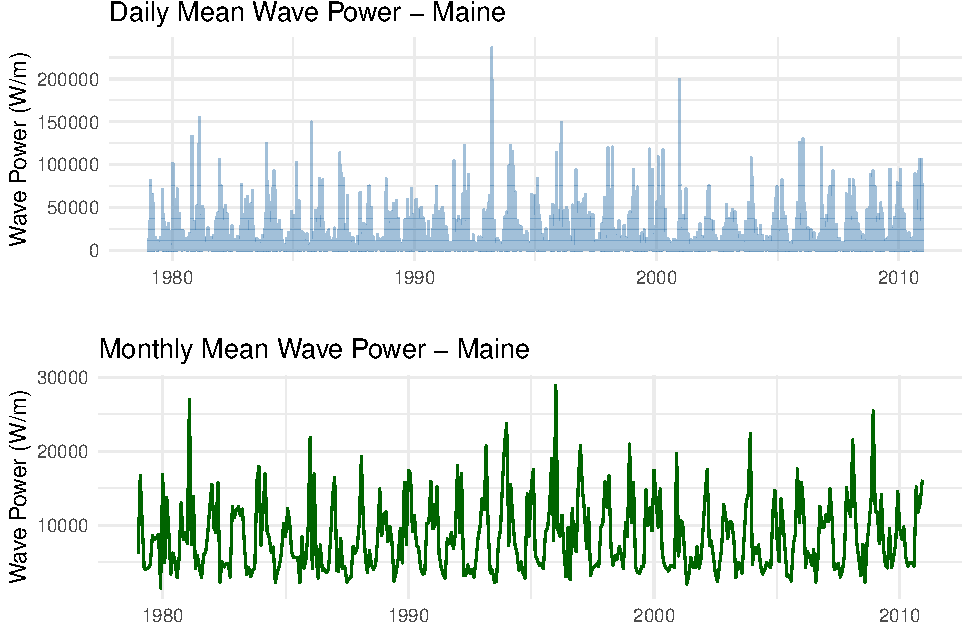
\includegraphics{Data_Cleaning_files/figure-latex/unnamed-chunk-8-1.pdf}
\includegraphics{Data_Cleaning_files/figure-latex/unnamed-chunk-8-2.pdf}
\includegraphics{Data_Cleaning_files/figure-latex/unnamed-chunk-8-3.pdf}

\includegraphics{Data_Cleaning_files/figure-latex/unnamed-chunk-9-1.pdf}

\begin{verbatim}
## Series: maine_ts_train 
## ARIMA(2,0,0)(2,0,0)[12] with non-zero mean 
## 
## Coefficients:
##           ar1     ar2    sar1    sar2       mean
##       -0.0136  0.1167  0.2955  0.3082  8431.9324
## s.e.   0.0661  0.0606  0.0573  0.0589   622.8468
## 
## sigma^2 = 17720534:  log likelihood = -2929.12
## AIC=5870.23   AICc=5870.52   BIC=5892.45
\end{verbatim}

\includegraphics{Data_Cleaning_files/figure-latex/unnamed-chunk-9-2.pdf}
\includegraphics{Data_Cleaning_files/figure-latex/unnamed-chunk-9-3.pdf}
\includegraphics{Data_Cleaning_files/figure-latex/unnamed-chunk-9-4.pdf}

\includegraphics{Data_Cleaning_files/figure-latex/unnamed-chunk-10-1.pdf}

\begin{verbatim}
## 
##  Ljung-Box test
## 
## data:  Residuals
## Q* = 18.166, df = 24, p-value = 0.7949
## 
## Model df: 0.   Total lags used: 24
\end{verbatim}

\includegraphics{Data_Cleaning_files/figure-latex/unnamed-chunk-10-2.pdf}
Model intial interpretation: - Residuals kind of fluctuate around 0, but
the variance is not very constant, but variance have slightly higher
value fluctuations \textgreater{} 0, so some inconsistency with
potential minor outliers. - ACF plot: no significant spikes outside of
the blue lines, which is good - Histogram of residuals display rough
normal distribution around 0, which is good. - Ljung-Box test: p-value
(0.79) much greater than 0.05, so residuals are white noise, good.

ACF: since the present value has very low correlation with the previous
periods in the short term. Since we are looking at tidal power,
longer-term trends may be more important, so es model did not do well.

\includegraphics{Data_Cleaning_files/figure-latex/unnamed-chunk-11-1.pdf}

\begin{verbatim}
## 
##  Ljung-Box test
## 
## data:  Residuals from StructTS
## Q* = 678.76, df = 24, p-value < 2.2e-16
## 
## Model df: 0.   Total lags used: 24
\end{verbatim}

\includegraphics{Data_Cleaning_files/figure-latex/unnamed-chunk-11-2.pdf}
This model without changes from Module 10 was bad, strong
autocorrelation and convergence issue, let's change:

\begin{verbatim}
## Warning in StructTS(maine_ts_train_diff, type = "BSM", , fixed = c(NA, NA, :
## possible convergence problem: 'optim' gave code = 52 and message 'ERROR:
## ABNORMAL_TERMINATION_IN_LNSRCH'
\end{verbatim}

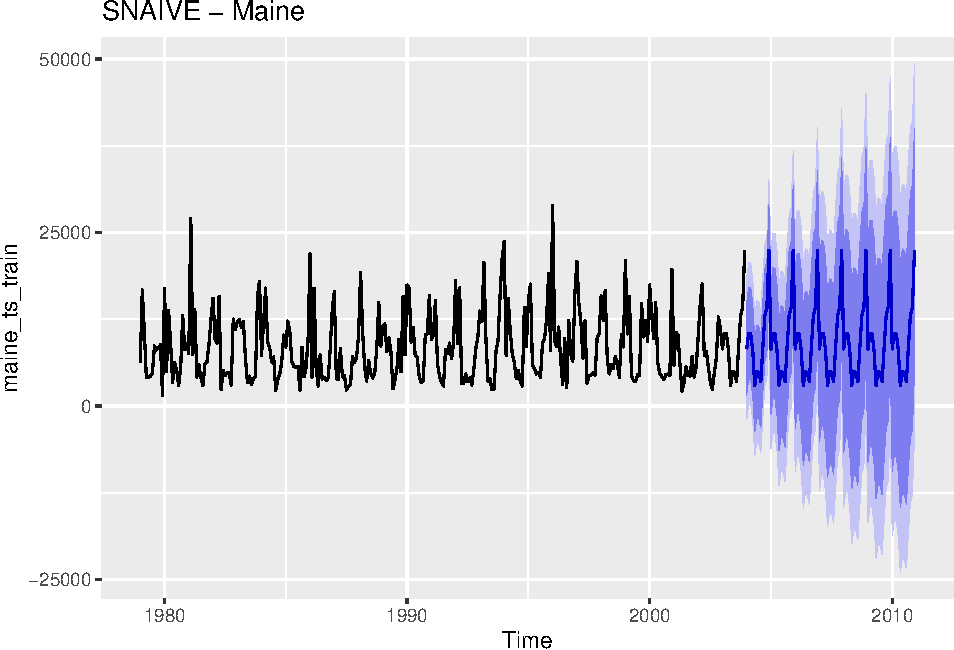
\includegraphics{Data_Cleaning_files/figure-latex/unnamed-chunk-12-1.pdf}

\begin{verbatim}
## 
##  Ljung-Box test
## 
## data:  Residuals from StructTS
## Q* = 101.35, df = 24, p-value = 1.764e-11
## 
## Model df: 0.   Total lags used: 24
\end{verbatim}

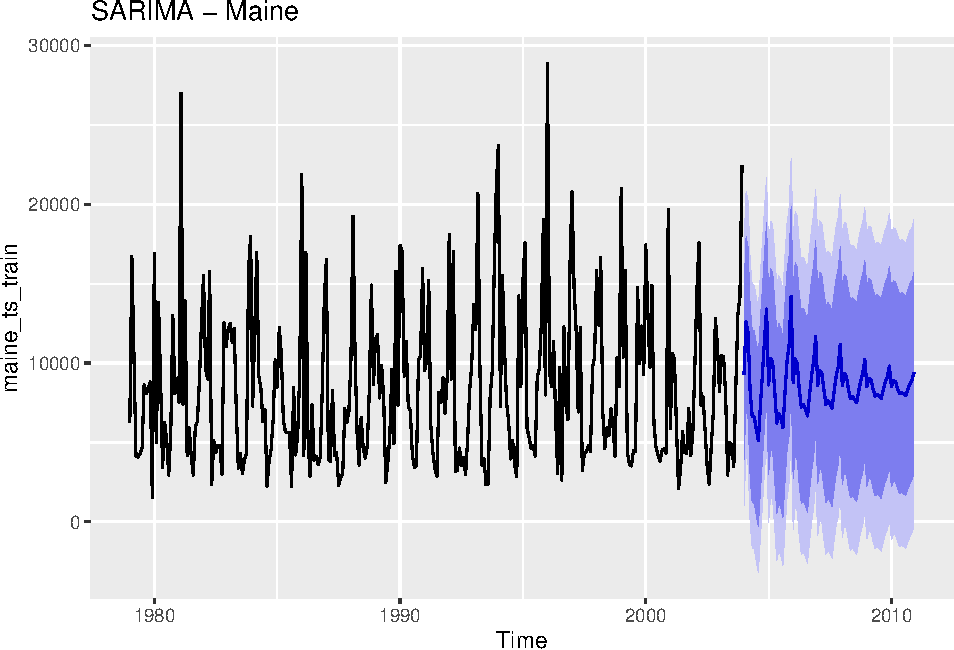
\includegraphics{Data_Cleaning_files/figure-latex/unnamed-chunk-12-2.pdf}
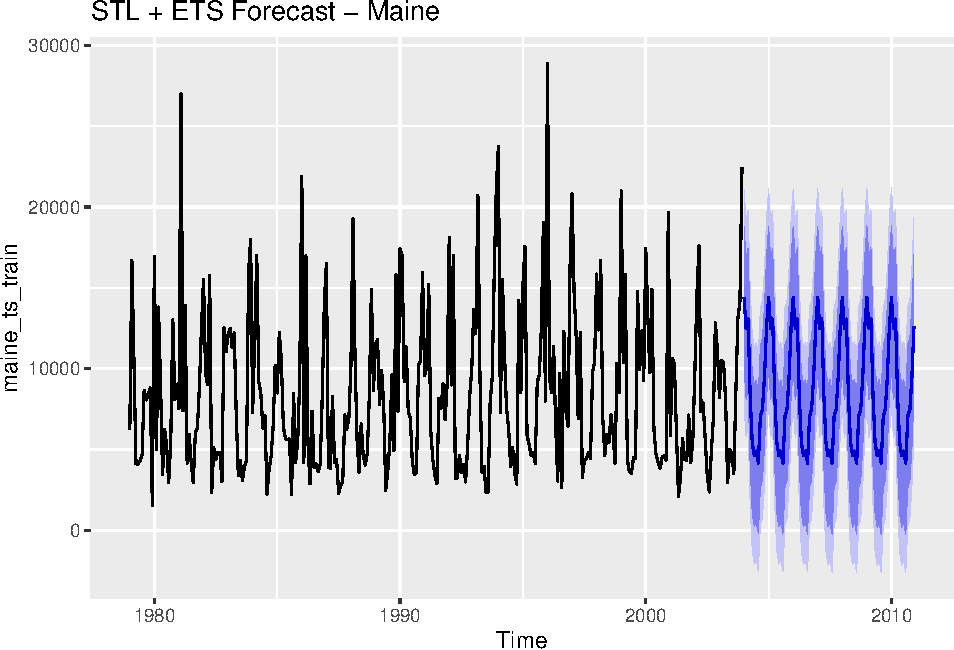
\includegraphics{Data_Cleaning_files/figure-latex/unnamed-chunk-12-3.pdf}
Revised model: Residual plot improvements (no trends/outliers) suggest:

\begin{itemize}
\item
  The model handles mean and variance reasonably well.
\item
  The seasonal/trend components are likely adequate.
\end{itemize}

ACF spikes + low p-value imply:

\begin{itemize}
\item
  Short-term dependencies remain unmodeled (e.g., AR/MA effects).
\item
  Seasonal harmonics (higher-frequency cycles) may be missed.
\end{itemize}

Next steps could be: - combine the StructTS model with arima layer

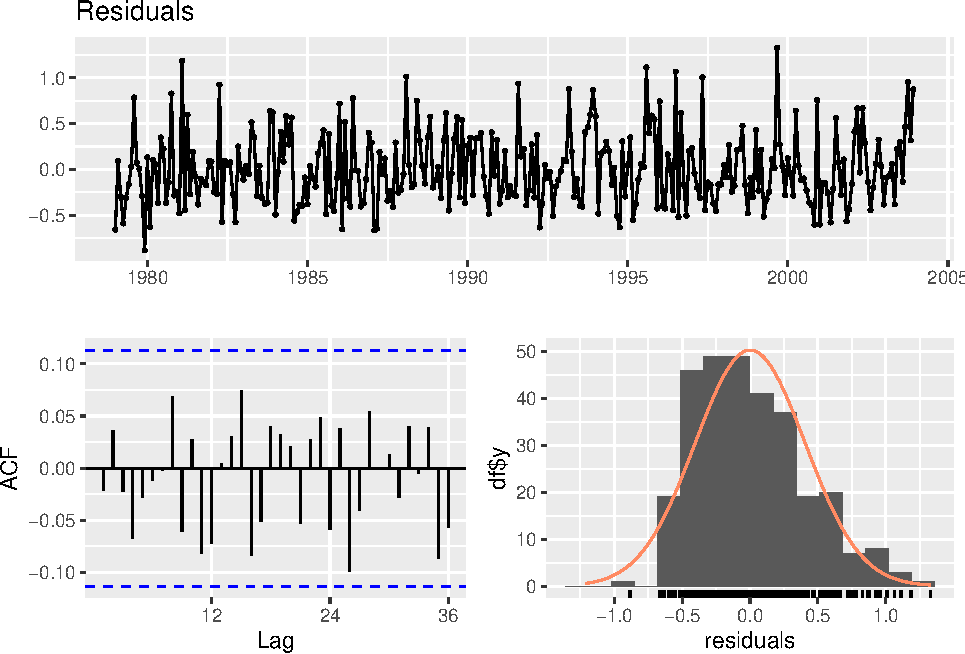
\includegraphics{Data_Cleaning_files/figure-latex/unnamed-chunk-13-1.pdf}
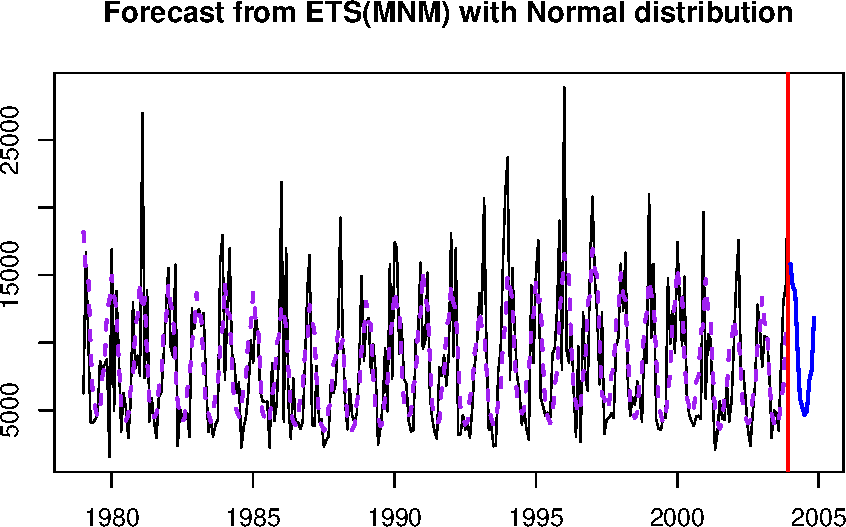
\includegraphics{Data_Cleaning_files/figure-latex/unnamed-chunk-13-2.pdf}

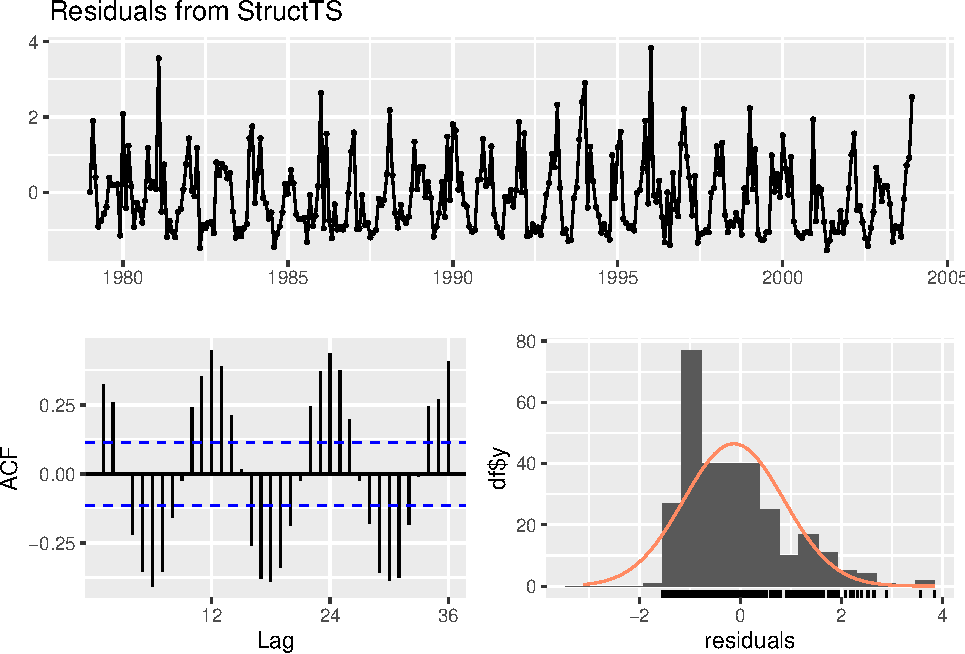
\includegraphics{Data_Cleaning_files/figure-latex/unnamed-chunk-14-1.pdf}
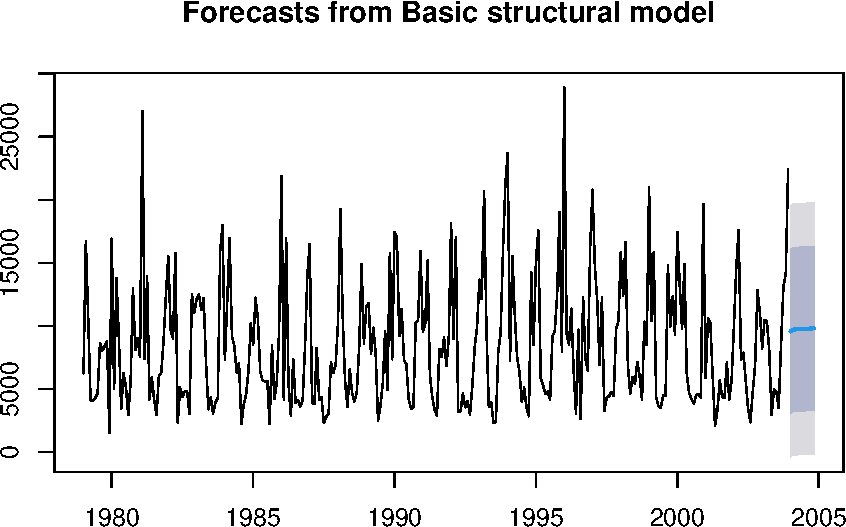
\includegraphics{Data_Cleaning_files/figure-latex/unnamed-chunk-14-2.pdf}

\begin{quote}
Observations: Both TBATS and NN under-forecast monthly tidal power.
TBATS performs slightly better but both models do not seem to capture
the seasonality of the monthly tidal power. For NN, some tweaking can be
done to see if changing the lag can better capture the seasonality.
\end{quote}

\begin{verbatim}
## The best model by RMSE is: ARIMA+Fourier
\end{verbatim}

\begin{table}[!h]
\centering\centering
\caption{\label{tab:unnamed-chunk-15}Forecast Accuracy for Monthly Wave Power - Maine}
\centering
\begin{tabular}[t]{l|r|r|r|r|r|r|r}
\hline
  & ME & RMSE & MAE & MPE & MAPE & ACF1 & Theil's U\\
\hline
SNAIVE & -822.5207 & 4290.692 & 3202.526 & -19.62825 & 42.60721 & 0.06549 & 0.89498\\
\hline
SARIMA & -217.5947 & 4026.117 & 3221.739 & -29.70686 & 50.01054 & 0.32049 & 0.83462\\
\hline
STL+ETS & -192.9789 & 3730.735 & 2709.232 & -17.21843 & 36.39588 & 0.18831 & 0.70042\\
\hline
\cellcolor{gray!10}{ARIMA+Fourier} & \cellcolor{gray!10}{736.3832} & \cellcolor{gray!10}{3690.025} & \cellcolor{gray!10}{2601.569} & \cellcolor{gray!10}{-5.30294} & \cellcolor{gray!10}{31.99013} & \cellcolor{gray!10}{0.20083} & \cellcolor{gray!10}{0.72561}\\
\hline
ES & 4686.0140 & 5864.526 & 4762.718 & 78.82107 & 80.54519 & -0.00122 & 1.84991\\
\hline
StructTS & 4686.0140 & 5864.526 & 4762.718 & 78.82107 & 80.54519 & -0.00122 & 1.84991\\
\hline
TBAT & 569.0860 & 3728.780 & 2690.142 & -8.37019 & 33.99924 & 0.17281 & 0.70592\\
\hline
NN & -184.8396 & 4066.413 & 2895.310 & -15.97632 & 38.23628 & 0.19439 & 0.75016\\
\hline
\end{tabular}
\end{table}

\#Alaska

\#\#\#Start by creating monthly time series objects for Alaska and
plotting ACF and PACF plots
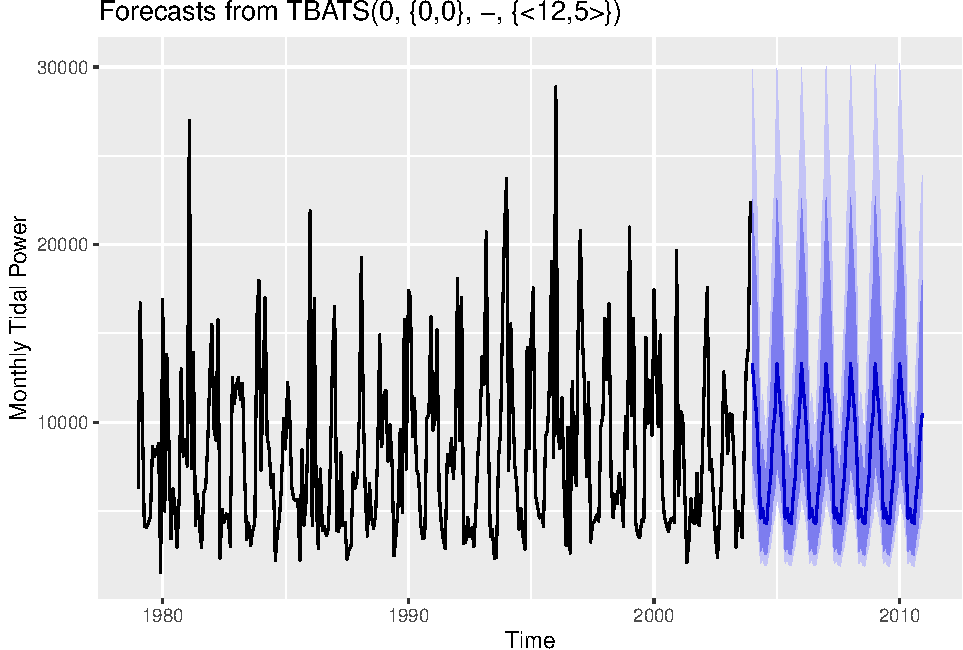
\includegraphics{Data_Cleaning_files/figure-latex/unnamed-chunk-16-1.pdf}
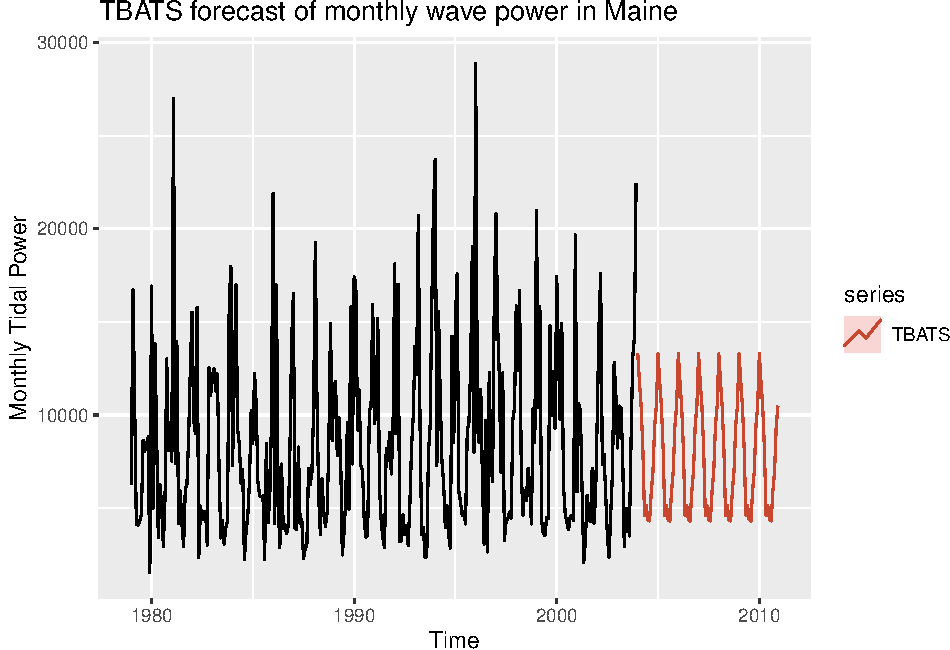
\includegraphics{Data_Cleaning_files/figure-latex/unnamed-chunk-16-2.pdf}
\includegraphics{Data_Cleaning_files/figure-latex/unnamed-chunk-16-3.pdf}

\begin{quote}
Observations: The significant spike at lag 1 in both ACF and PACF
strongly suggests an AR(1) component. Also, the significant spikes at
lag 12 in both ACF and PACF indicate a strong seasonal autoregressive
component with a period of 12 months (SAR(1) with a seasonal lag of 12).
\end{quote}

\begin{verbatim}
## Warning in adf.test(alaska_ts_train): p-value smaller than printed p-value
\end{verbatim}

\begin{verbatim}
## 
##  Augmented Dickey-Fuller Test
## 
## data:  alaska_ts_train
## Dickey-Fuller = -7.3596, Lag order = 6, p-value = 0.01
## alternative hypothesis: stationary
\end{verbatim}

\begin{quote}
Observations: ADF test returns a p-value of 0.01, which is smaller than
our chosen significance level of 0.05. We reject the null hypothesis
that the Alaska mean monthly wave power series has a unit root and thus,
the series is likely stationary and does not need differencing.
\end{quote}

\#\#\#Proceed with using our 3 chosen models on Alaska \#\# Model 1: STL
decomposition + ETS
\includegraphics{Data_Cleaning_files/figure-latex/unnamed-chunk-18-1.pdf}

\subsection{Model 2: ARIMA + Fourier
terms}\label{model-2-arima-fourier-terms}

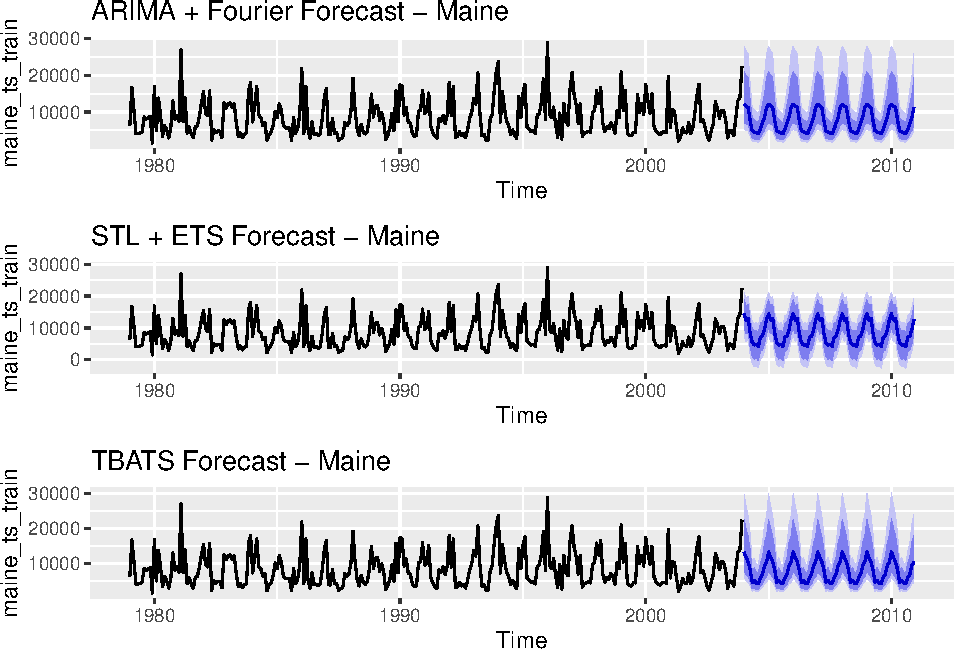
\includegraphics{Data_Cleaning_files/figure-latex/unnamed-chunk-19-1.pdf}

\subsection{Model 3: TBATS}\label{model-3-tbats}

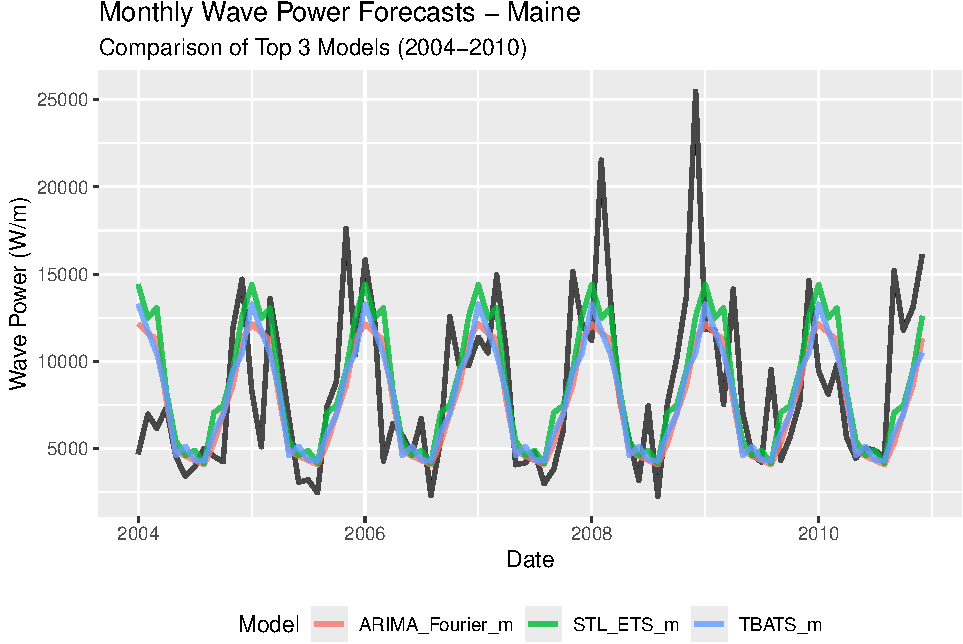
\includegraphics{Data_Cleaning_files/figure-latex/unnamed-chunk-20-1.pdf}
\includegraphics{Data_Cleaning_files/figure-latex/unnamed-chunk-20-2.pdf}

\begin{verbatim}
## The best model by RMSE is: ARIMA+Fourier
\end{verbatim}

\begin{table}[!h]
\centering\centering
\caption{\label{tab:unnamed-chunk-21}Forecast Accuracy for Monthly Wave Power - alaska}
\centering
\begin{tabular}[t]{l|r|r|r|r|r|r|r}
\hline
  & ME & RMSE & MAE & MPE & MAPE & ACF1 & Theil's U\\
\hline
STL+ETS & 0.41065 & 14.12462 & 10.06050 & -118.37052 & 148.4886 & 0.24409 & 0.44005\\
\hline
\cellcolor{gray!10}{ARIMA+Fourier} & \cellcolor{gray!10}{2.70368} & \cellcolor{gray!10}{13.68095} & \cellcolor{gray!10}{9.00760} & \cellcolor{gray!10}{-79.91860} & \cellcolor{gray!10}{115.1316} & \cellcolor{gray!10}{0.19990} & \cellcolor{gray!10}{0.39252}\\
\hline
TBAT & 3.71047 & 14.20461 & 8.81815 & -71.65192 & 107.4045 & 0.18163 & 0.41341\\
\hline
\end{tabular}
\end{table}

\#Florida

\#\#\#Start by creating monthly time series objects for Florida and
plotting ACF and PACF plots
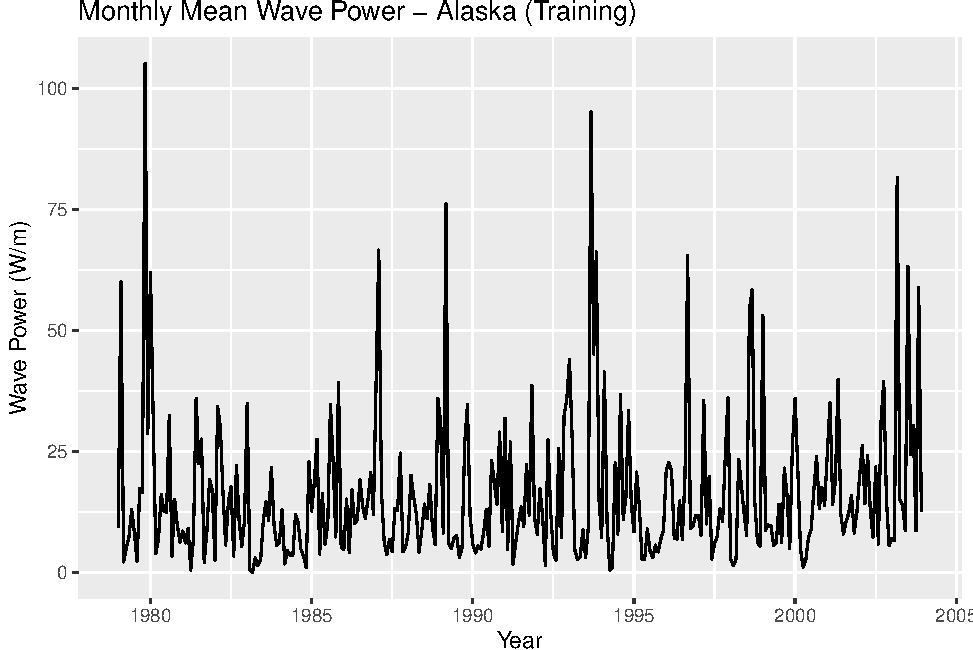
\includegraphics{Data_Cleaning_files/figure-latex/unnamed-chunk-22-1.pdf}
\includegraphics{Data_Cleaning_files/figure-latex/unnamed-chunk-22-2.pdf}
\includegraphics{Data_Cleaning_files/figure-latex/unnamed-chunk-22-3.pdf}

\begin{quote}
Observations: The significant spike at lag 1 in both ACF and PACF
strongly suggests an AR(1) component. Also, the repeating seasonal
patterns at lag 12 for the ACF suggest strong yearly seasonality.
\end{quote}

\begin{verbatim}
## Warning in adf.test(florida_ts_train): p-value smaller than printed p-value
\end{verbatim}

\begin{verbatim}
## 
##  Augmented Dickey-Fuller Test
## 
## data:  florida_ts_train
## Dickey-Fuller = -12.062, Lag order = 6, p-value = 0.01
## alternative hypothesis: stationary
\end{verbatim}

\begin{quote}
Observations: ADF test returns a p-value of 0.01, which is smaller than
our chosen significance level of 0.05. We reject the null hypothesis
that the Alaska mean monthly wave power series has a unit root and thus,
the series is likely stationary and does not need differencing.
\end{quote}

\#\#\#Proceed with using our 3 chosen models on Florida
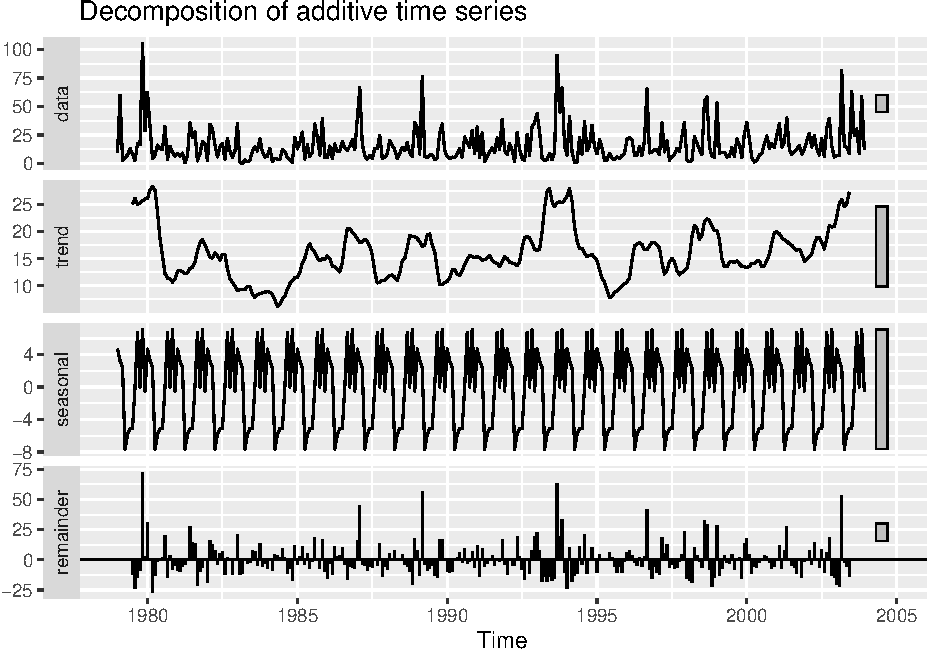
\includegraphics{Data_Cleaning_files/figure-latex/unnamed-chunk-24-1.pdf}

\subsection{Model 2: ARIMA + Fourier
terms}\label{model-2-arima-fourier-terms-1}

\includegraphics{Data_Cleaning_files/figure-latex/unnamed-chunk-25-1.pdf}

\subsection{Model 3 TBATs}\label{model-3-tbats-1}

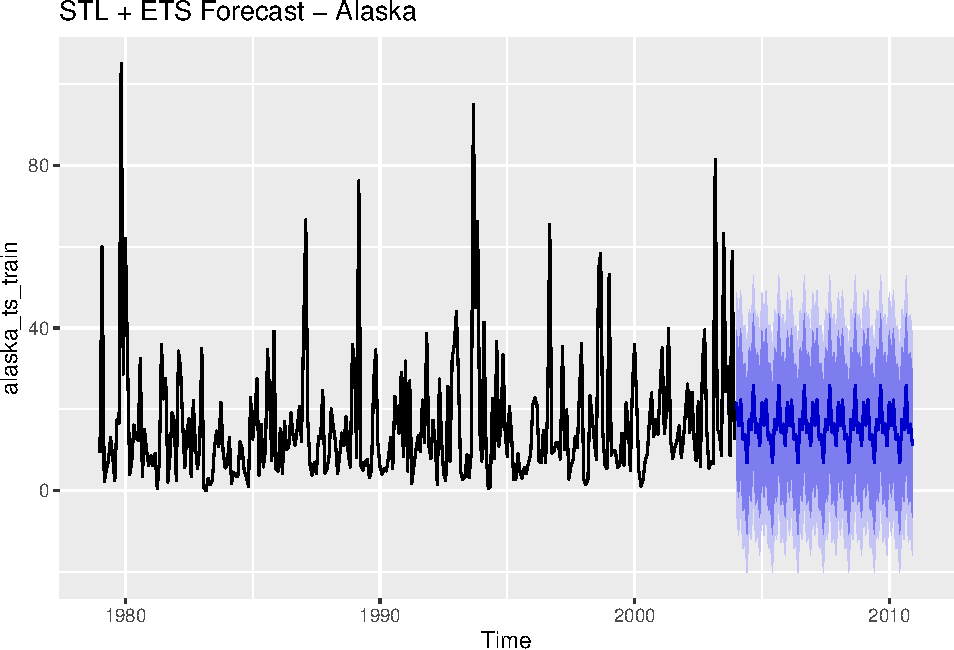
\includegraphics{Data_Cleaning_files/figure-latex/unnamed-chunk-26-1.pdf}
\includegraphics{Data_Cleaning_files/figure-latex/unnamed-chunk-26-2.pdf}

\begin{verbatim}
## The best model by RMSE is: STL+ETS
\end{verbatim}

\begin{table}[!h]
\centering\centering
\caption{\label{tab:unnamed-chunk-27}Forecast Accuracy for Monthly Wave Power - Florida}
\centering
\begin{tabular}[t]{l|r|r|r|r|r|r|r}
\hline
  & ME & RMSE & MAE & MPE & MAPE & ACF1 & Theil's U\\
\hline
\cellcolor{gray!10}{STL+ETS} & \cellcolor{gray!10}{260.0615} & \cellcolor{gray!10}{1884.797} & \cellcolor{gray!10}{1242.601} & \cellcolor{gray!10}{-22.94636} & \cellcolor{gray!10}{48.47699} & \cellcolor{gray!10}{0.04601} & \cellcolor{gray!10}{0.78809}\\
\hline
ARIMA+Fourier & 377.5698 & 2019.667 & 1254.629 & -13.78776 & 42.55154 & 0.03404 & 0.85821\\
\hline
TBAT & 644.5316 & 2081.479 & 1271.549 & -4.49300 & 39.17815 & 0.02116 & 0.86973\\
\hline
\end{tabular}
\end{table}

\end{document}
